\section{Analysis and Results}
\label{section:analysis}

\subsection{Scenarios}
- Benchmark: a lot of corners with minimal amount of obstacles\\
- Spiral: Also many corners, minimal distance\\
- SF: real world grid. Many obstacles, corners nearly always 90 degrees. Very predictable for algorithm\\
- Leuven: real world and irregular. Even more obstacles. Very unpredictable\\

To test the complete algorithm, several different scenarios have been used. Each scenario has unique characteristics and was tested with two different problem sizes. Theta* is always executed with a grid size of 2m and each time step has a duration of 200ms. All tests were executed on an Intel Core i5-4690k running at 4.4GHz with 16GB of 1600MHz DDR3 memory. The reported times are averages of 5 runs. The machine runs on Windows 10 using version 12.6 of IBM CPLEX. Figure \ref{fig:scenarios} shows these scenarios visually. Table \ref{table:results} shows detailed information about the scenarios and execution times.

\subsubsection{Up/Down Scenario}
The first test scenario has very few obstacles, but lays them out in a way such that the vehicle needs to slalom around them. The small scenario has only 5 obstacles, while the larger one has 9. This is a very challenging scenario for MILP because every obstacle has a large impact on the path. Without segmentation on the version of the scenario, the solver does not find the optimal path within 30 minutes. If execution is limited to 10 minutes, the best solution it finds takes 26.0s to execute by the vehicle. That is less than a second faster than the segmented result while it took more than 20 times more execution time to find that solution. For the larger scenario with 9 obstacles, the solver could not find a solution within 30 minutes. This scenario clearly shows the advantages of segmentation, even if there only are a few obstacles.

\subsubsection{San Francisco Scenario}
The San Francisco scenario covers a 1km by 1km section of the city for the small scenario, and 3km by 3km section for the large scenario. All the obstacles in this scenario are grid-aligned rectangles laid out in typical city blocks. Because of this, density of obstacles is predictable. This scenario showcases that the algorithm can scale to realistic scenarios with much more obstacles than is typically possible with a MIP approach. With these constraints, parameters and hardware, the path can be planned faster than the vehicle can execute it.

\subsubsection{Leuven Scenario}
The Leuven scenario also covers both a 1km by 1km and 3km by 3km section, this time of the Belgian city of Leuven. This is an old city with a very irregular layout. The dataset, provided by the local government\footnote{\url{https://overheid.vlaanderen.be/producten-diensten/basiskaart-vlaanderen-grb}}, also contains full polygons instead of the grid-aligned rectangles of the San Francisco dataset. While most buildings in the city are low enough so a UAV could fly over, it presents a very difficult test case for the path planning algorithm. The density of obstacles varies greatly and is much higher than in the San Francisco dataset across the board. The algorithm does slow down, but it is still fast enough for offline planning. As visible in figure \ref{fig:pre-3-4}, there are many obstacles clustered close to each other, with many edges being completely redundant. For a real application, a small amount of preprocessing of the map data should be able to significantly reduce both the amount of obstacles as the amount of edges. 

\begin{figure}
	\centering
	
	\begin{subfigure}[t]{0.74\textwidth}
        		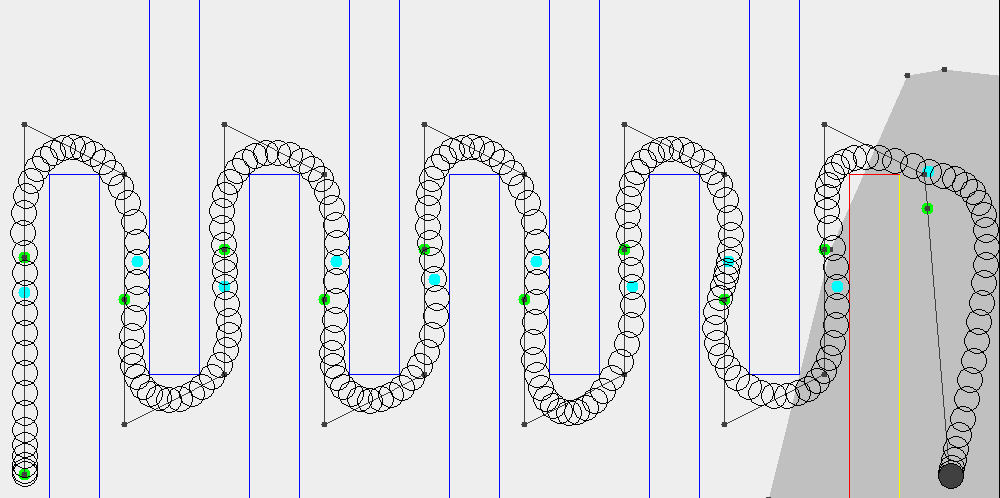
\includegraphics[width=\textwidth]{img/benchmarkfull}
        		\caption{}
	\end{subfigure}
		
	\begin{subfigure}[t]{0.70\textwidth}
        		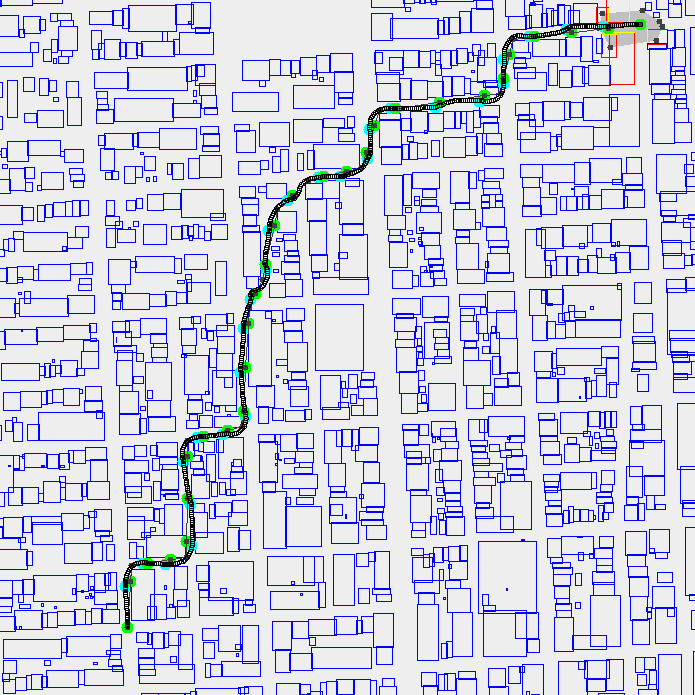
\includegraphics[width=\textwidth]{img/SF}
        		\caption{}
	\end{subfigure}	
	
	\begin{subfigure}[t]{0.70\textwidth}
        		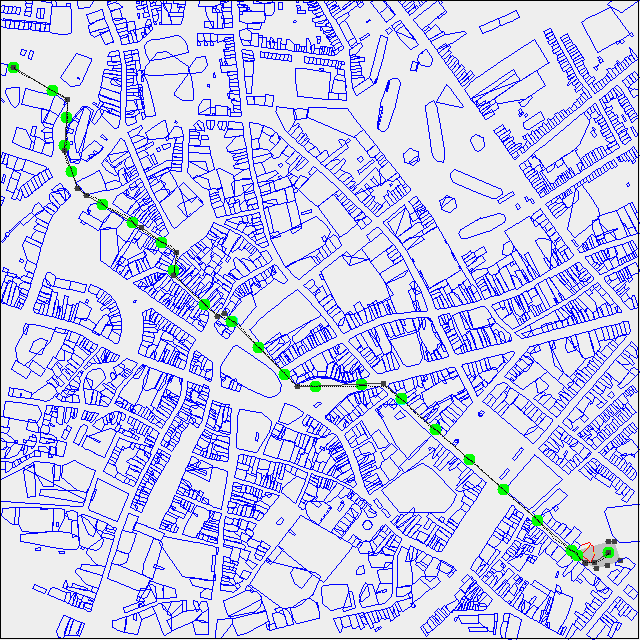
\includegraphics[width=\textwidth]{img/leuven}
        		\caption{}
	\end{subfigure}
        
    \caption{These are the three different worlds which were tested. The top image shows the large Up/Down scenario. The middle image shows the small San Francisco scenario. Note how the obstacles are only grid-aligned rectangles laid out in a grid pattern. The bottom image shows the small Leuven scenario. The obstacles are polygons and distributed in a much more irregular pattern compared to the San Francisco scenario.}\label{fig:scenarios}
\end{figure}


\begin{figure}
\begin{tabular}{ l l l l l l l l l }
 scenario & \# obstacles & world size & path length & \# segments & Theta* time & Gen. Al. time & MILP time & score \\ 
 \hline
Up/Down Small & 5 &  25m x 20m & 88m  & 7 & 0.09s & 1.10s & 20.8s & 26.6s\\
Up/Down Large & 9 & 40m x 20m &  146m & 11 & 0.14s & 1.62s & 40.1s & 43.6s \\
SF Small & 684 & 1km x 1km & 1392m & 28 & 2.04s & 9.56s & 59.2s & 105.7s \\
SF Large & 6580 & 3km x 3km & 4325m  & 84 & 18.14s & 18.21s & 231s & 316.0s\\
Leuven Small & 3079 & 1km x 1km & 1312m & 29 &  2.29s & 29.83s & 152s  & 95.9s \\
Leuven Large & 18876 & 3km x 3km & 3041m & 61 & 18.14s & 83.69s & 687s & 217.6s \\

\end{tabular}
\caption{The experimental results for the different scenarios}
\label{table:results}
\end{figure}
\subsection{Convexity of Search Space}
The convexity of the search space plays a large role in the difficulty of a MILP problem. My approach is built entirely around the idea of keeping the search space as convex as possible in each segment. To analyze  the importance of convexity, I tested three scenarios without any form of preprocessing. These scenarios are designed so the optimal trajectory has roughly the same duration in each scenario. The scenarios also each have 5 grid aligned rectangles as obstacles.\\
As a result, MILP problems for all three scenarios have nearly identical amounts of integer variables. The difference between these scenarios is the convexity of the search space. \\
In the first scenario, the obstacles are not in the way of the UAV. The UAV can move in a straight line from the start position to its goal. In the second scenario, two of the obstacles are slightly in the way. The UAV is forced to make slight turns near the start and end of the trajectory. However, most of the trajectory is still straight. In the third scenario, the vehicle has to slalom around every obstacle.\\

\subsubsection{Results}
TODO: ADD RESULTS\\
TODO: ADD IMAGES \\
\subsubsection{Interpretation}
Even though all scenarios have nearly identical amounts of time steps, integer variables and obstacles, the solve time varies greatly. This confirms the core assumption behind my approach: The convexity of the search space plays a larger role in the performance than the amount of integer variables.





\subsection{Genetic Algorithm Parameters}
tweak parameters...




\subsection{Agility of the UAV}
The properties of the segments strongly rely on the agility of the UAV. The size of the segments is determined by the maximum acceleration distance of the UAV. This is the distance the UAV needs to accelerate from zero to its maximum velocity, or decelerate from the maximum velocity to zero. \\
In this experiment, I tested relation between the maximum velocity and the maximum acceleration of the UAV. I used the large Up/Down scenario, the small San Francisco scenario and the small Leuven scenario. For each scenario I tested nine configurations of the vehicle: Every combination between three different maximum velocities and three different maximum accelerations.\\
TODO: add \# segments

\begin{figure}
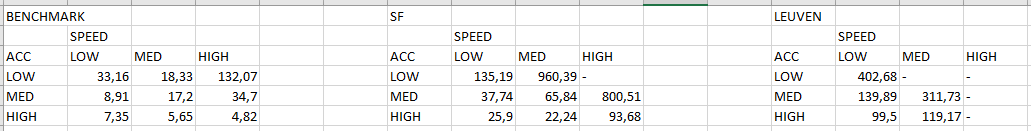
\includegraphics[width=\textwidth]{img/agility1}
caption{}
\label{fig:agility-times}
\end{figure}
Even though some combinations did not finish for the larger scenarios, the results are relatively consistent across all three scenarios:\\
Within each speed category, a higher acceleration always reduces solve times. This is as expected, because a higher acceleration will reduce the expansion distance for the segments, making them both shorter in time as well as smaller so less obstacles are expected to be modeled.\\
Increasing the velocity for the low and medium acceleration tends to make things slower.
Low velocity and high acceleration always score well







\subsection{Cornercutting}
A trajectory that allows corner cutting cannot be considered safe. However, additional constraints are required to prevent this from happening. This experiment attempts to measure the impact of the corner cutting prevention.


\subsubsection{Result}
\begin{figure}
CORNER CUT
% 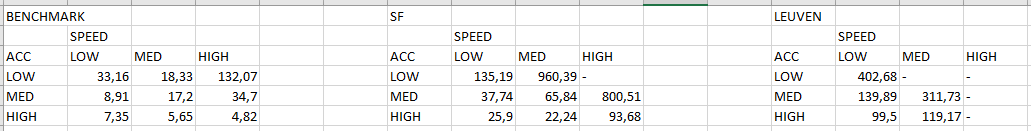
\includegraphics[width=\textwidth]{img/agility1}
caption{}
\label{fig:corner-data}
\end{figure}

The performance impact caused by preventing corner cutting seems minimal (TODO: more precise!).



\subsection{Linear approximation}
The velocity and acceleration of the UAV are limited to some finite value. Because both of those quantities are vectors, that maximum can only be approximated with linear constraints. More constraints are needed to model this more accurately which can allow for faster solutions. However, more constraints also have a performance cost. This experiment analyses the trade-off that needs to be made.
\begin{figure}
LINEAR APPROX
% 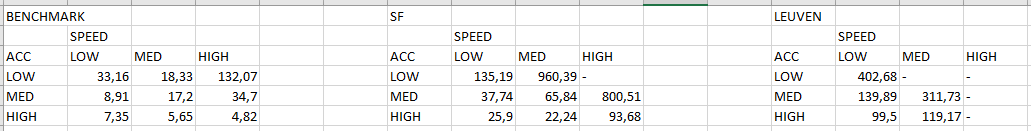
\includegraphics[width=\textwidth]{img/agility1}
caption{}
\label{fig:linear-approx-data}
\end{figure}


\subsection{Time step size}
The time step size determines how many time steps are used in each MILP problem. A smaller step sizes allows for better results, but at a performance cost

\begin{figure}
TIME STEP
% 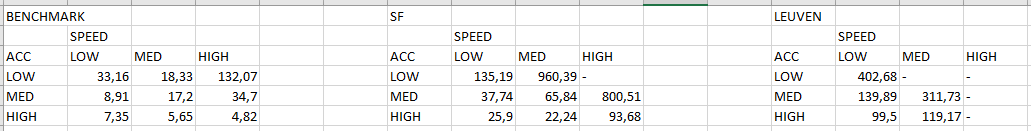
\includegraphics[width=\textwidth]{img/agility1}
caption{}
\label{fig:timestep-data}
\end{figure}
The time step size has a dramatic impact on performance. For the benchmark scenario, each increase in the amount of time steps resulted in around 14x the computation time. For the San Francisco scenario, that is around 6-7x. In both cases the trajectory time improved with more time steps as well, although the difference is smaller when going from 5fps to 10fps compared to 2fps to 5fps.


\subsection{Stability}

\subsection{Max Time}

\subsection{Issues}

\subsubsection{Active region}
often good results, but sometimes cuts corner too close

\subsubsection{Segment transitions}
small epsilon -> uav needs to slow down, forces trajectory very close to path
large epsilon + line -> uav tends to curve and still slow down close to transition, cause unknown?
						-> cause: needs to be able to stop?                        
occasional failures: jerk only? TEST!!
transition itself is weak point of approach. Possible way to solve: resolve transition area based on a bit before and after transition

\subsubsection{Maximum time for segment}
Finding maximum time for a segment needs to overestimate: more time steps cause longer solve times
Solution: generate path at lower temporal resolution to find accurate time needed. Could improve solve time





% \subsection{Safety}
% guaranteed by constraints, however:\\
% no incentive to stay away from walls. Can increase vehicle size, but prevents occasionally getting closer for a short while.\\
% \subsection{Stability and Performance}
% -maxtime (max length of segment)\\
% - approach margin: larger -> better approach, longer solve time\\
% - tolerance: larger -> when corners are close, merge faster: more execution time\\
% - position tolerance: larger -> smoother path, strays further from preprocessed path so needs to backtrack more often\\
% - backtracking effect?\\
% -can quickly recalculate based on measured state? IMPLEMENT WARM START EXPERIMENT?\\


\section{Discussion}
The results show a large improvement in scalability in certain realistic scenarios, but the choice of those scenarios has drastically impacted the algorithm I have developed. \\
During development, I have always used realistic approximations of the capabilities of multirotor UAVs. Those can reach high accelerations but have relatively low maximum velocities compared to what fixed-wing aircraft can achieve. This makes those vehicles very agile, which is one of the contributing factors to their recent popularity. \\
Assuming this agility means that my algorithm cannot be applied to UAVs which do not have that property. One of the properties my algorithm uses often is the maximum acceleration distance, which is the distance in which the UAV can always come to a complete stop. This works fine with multirotor UAVs, but is a meaningless concept when dealing with fixed-wing UAVs which cannot stop at all during flight. \\
However, those kinds of low-agility UAVs are unlikely to be deployed at low altitudes in dense city centers exactly because they lack agility. Even with perfect planning, cities are very unpredictable places. An multirotor UAV is much more likely to be able to safely react to an unexpected obstacle than a fixed-wing UAV. \\
While I picked out fixed-wing UAVs as an example, the same arguments hold for any kind of UAV that either cannot hover or has low agility. Some UAVs may be able to hover, but are not very agile due to a high maximum velocity and low acceleration. In this case, the agility can be improved by reducing the maximum velocity.\\ \\

Another point that warrants attention are the transition between segments. In some cases, the UAV may end a segment in a state which causes issues in the next segment. This may cause the next segment to not be solvable, or result in a strange and undesirable trajectory. Overlapping the segments does help, but the algorithm can still not guarantee that the next segment will be feasible. Backtracking does guarantee that the next segment will be feasible, but at a great computational cost.\\
This is partly due to active region generated by the genetic algorithm. Often the results are good, but in some cases the active region is very restrictive. The algorithm itself could certainly be improved, but it will be hard to guarantee a good result. Forcing the region to be significantly large solves the issue, but that comes at computational cost that may be too large.\\

However, I do believe that these transition issues can be solved. One of the next extensions I would try is solving the MILP problem first with a higher time step size. Using this to roughly solve the current and next segment to provide a suitable goal state (including velocity) for the first segment would ensure a good start for the next segment as well. This may also allow for a lower approach margin multiplier, because the proper approach is already determined. \\

Another extension I would try is using moving to Mixed Integer Quadratic programming. Linear approximations to limit the length of vectors works, but it also introduces artifacts into the path. Increasing the amount of constraints that model the norm helps minimize the impact, but comes at a performance cost. Stating those constraints directly as a quadratic function would reduce the amount of constraints needed per time step. This could improve performance, and entirely eliminates the artifacts. Especially when the problem is also extended to 3D, since the this would require the linear approximation of a sphere instead of a circle. \\

The obvious next step is extending this approach to 3D. The extra degree of freedom will likely come at a significant performance penalty, so this was not attempted during the thesis. One of the likely difficulties with the preprocessing as presented is that it treats all dimensions the same. This is fine for the horizontal dimensions, but due to gravity, movements the vertical dimension have different characteristics. The maximum acceleration of the UAV can no longer be assumed to be the same in all directions.\\
A possible mitigation to the increasing complexity of obstacles may be using a "2.5D" representation. A 2.5D obstacle is a 2D obstacle which also has a height value. This would only need one additional integer variable per obstacle to model. In a city scenario, this may be an acceptable approximation. \\
% \subsection{Other weaknesses}
% waviness\\
% bad approaches to corners\\
% transitions between segments\\\\

% eigen abs:\\
% slack -> abs = val\\
% -slack -> abs = -val\\\\

% --> 2 vars voor abs\\\\

% abs norm:\\
% speed >= dot product[i]\\
% slack[i] -> speed = dot product[i]\\\\

% --> speed: num points / 4 vars\\\\

% norm:\\
% slack[i] and absslackx -> circle x\\
% slack[i] and - absslackx -> - circle x\\\\

% --> norm: geen extra vars   \\